%!TEX encoding = UTF-8 Unicode
%!TEX root = ../Main/thesis.tex
% !TEX spellcheck = en-US
%%=========================================
\documentclass[../Main/thesis.tex]{subfiles}
\begin{document}
\chapter{Literature Overview}
\label{ch:literature_overview}
This chapter presents a review of research that is relevant to this study. %of research and theory about existing technology and reviews similar research fields.
It is organized in three parts.
First, an account of how the study relates to the field of learning analytics is provided.
Second, an overview of existing positioning systems, both for indoor and outdoor positioning is presented.
Third a comparison of similar research projects is given.

\section{Learning Analytics} 
Learning analytics is described as using data about learning patterns and activity to provide new insights into educational practices and to improve learning, teaching and decision-making \citep{Siemens2012a}
At the \textit{1st International Conference on Learning Analytics \& Knowledge} in 2011 learning analytics was defined as: \textit{``Learning analytics is the measurement, collection, analysis and reporting of data about learners and their contexts, for purposes of understanding and optimising learning and the environments in which it occurs.''} \citep{BuckinghamShum2012}.
This is still the most common definition.
Often learning analytics is about utilizing existing data sources to enhance opportunities for learning.
Accordingly, this study is about utilizing data to improve practice.

\subsection*{Multimodal Learning Analytics}
Multimodal Learning Analytics is described as using multiple data sources for extracting data from a learning situation, to predict, understand, and quantify student learning \citep{Worsley2010}.
It has later been defined by \citet{Worsley2016} as: \textit{``Multimodal learning analytics (MMLA) sits at the intersection of three ideas: multimodal teaching and learning, multimodal data, and computer-supported analysis. At its essence, MMLA utilizes and triangulates among non-traditional as well as traditional forms of data in order to characterize or model student learning in complex learning environments.''}
While learning analytics often is about utilizing existing data sources, e.g. from university student administrative systems, it can also be about purposefully designing data sources to be used to improve learning as an integral part of the design of the learning activity. 
For example, \citet{Spikol2016} have designed a system for using learning analytics for supporting hands-on engineering design tasks.
\citet{Echeverria2018} have combined role-based nurses' movement data with high fidelity patient manikin logs to implement a zone-based classification model and visualize movements within an emergency response team, which provides the data needed to give real-time feedback for both students and instructors.
The research presented in this thesis uses multimodal data.

\section{Positioning Systems}
The literature on positioning systems can be split in two categories: outdoor positioning and indoor positioning.

\subsection{Outdoor positioning}
GNSS enables outdoors positioning.
They can provide global or local coverage.
There are several infrastructures that provide positioning data for example GPS, GLONASS, Galileo, and BeiDou.
The Global Positioning System (GPS) is owned by the United States Government and consists of 24 satellites and delivers worldwide positioning, navigation and timing \citep{U.S.DepartmentofDefence2008}.
GPS provides an general outdoor accuracy of three meter horizontally and five meter vertically in most situations \citep{U.S.DepartmentofDefence2008}, and with mobile phones the horizontal accuracy is between 5.0m and 8.5m \citep{Zandbergen2011a}.
This limit on accuracy itself would limit the usability of GPS indoors.
As GPS demands a free line of sight from the device to four or more satellites, the indoor precision is even less accurate \citep{Zandbergen2011a}.

Today GPS is available for a very large part of the population as GPS chips are embedded in most smartphones, and it would be convenient to be able to use it for indoor tracking as well, but because of the lack of indoor precision the use case is very limited.

GLONASS (Global Navigation Satellite System) is an alternative to GPS owned by the Russian Federation \citep{InformationandAnalysisCenterforPositioningNavigationandTiming2018}.
It consists of 26 satellites which covers the globe \citep{InformationandAnalysisCenterforPositioningNavigationandTiming2018a}.
According to \citet{Russiansystemofdifferentionalcorrectionandmonitoring2018} the outdoor horizontal accuracy of GLONASS, as of November 22 2018, is between 4 meters and 18 meters.
Indoors GLONASS suffers from the same inaccuracy as GPS because of the obstruction of signals.

\subsection{Indoor positioning}
\label{sec:indoor-positioning}
Indoor positioning systems (IPS) are systems for positioning an object inside a building.
Generally such systems can provide either low accuracy over a large area or high accuracy in a small area.
Systems that provide high accuracy often require extensive infrastructure, many sensors and time consuming calibration \citep{Curran2011}.
Indoor positioning systems can use a variety of technologies, such as WiFi \citep{chang2010robust}, Radio frequency identification (RFID) \citep{Saab2011}, light \citep{xiaohan2010improved}, sound \citep{schweinzer2010ultrasonic}, or Bluetooth, to achieve positioning.

\begin{figure}[h]
	\centering
	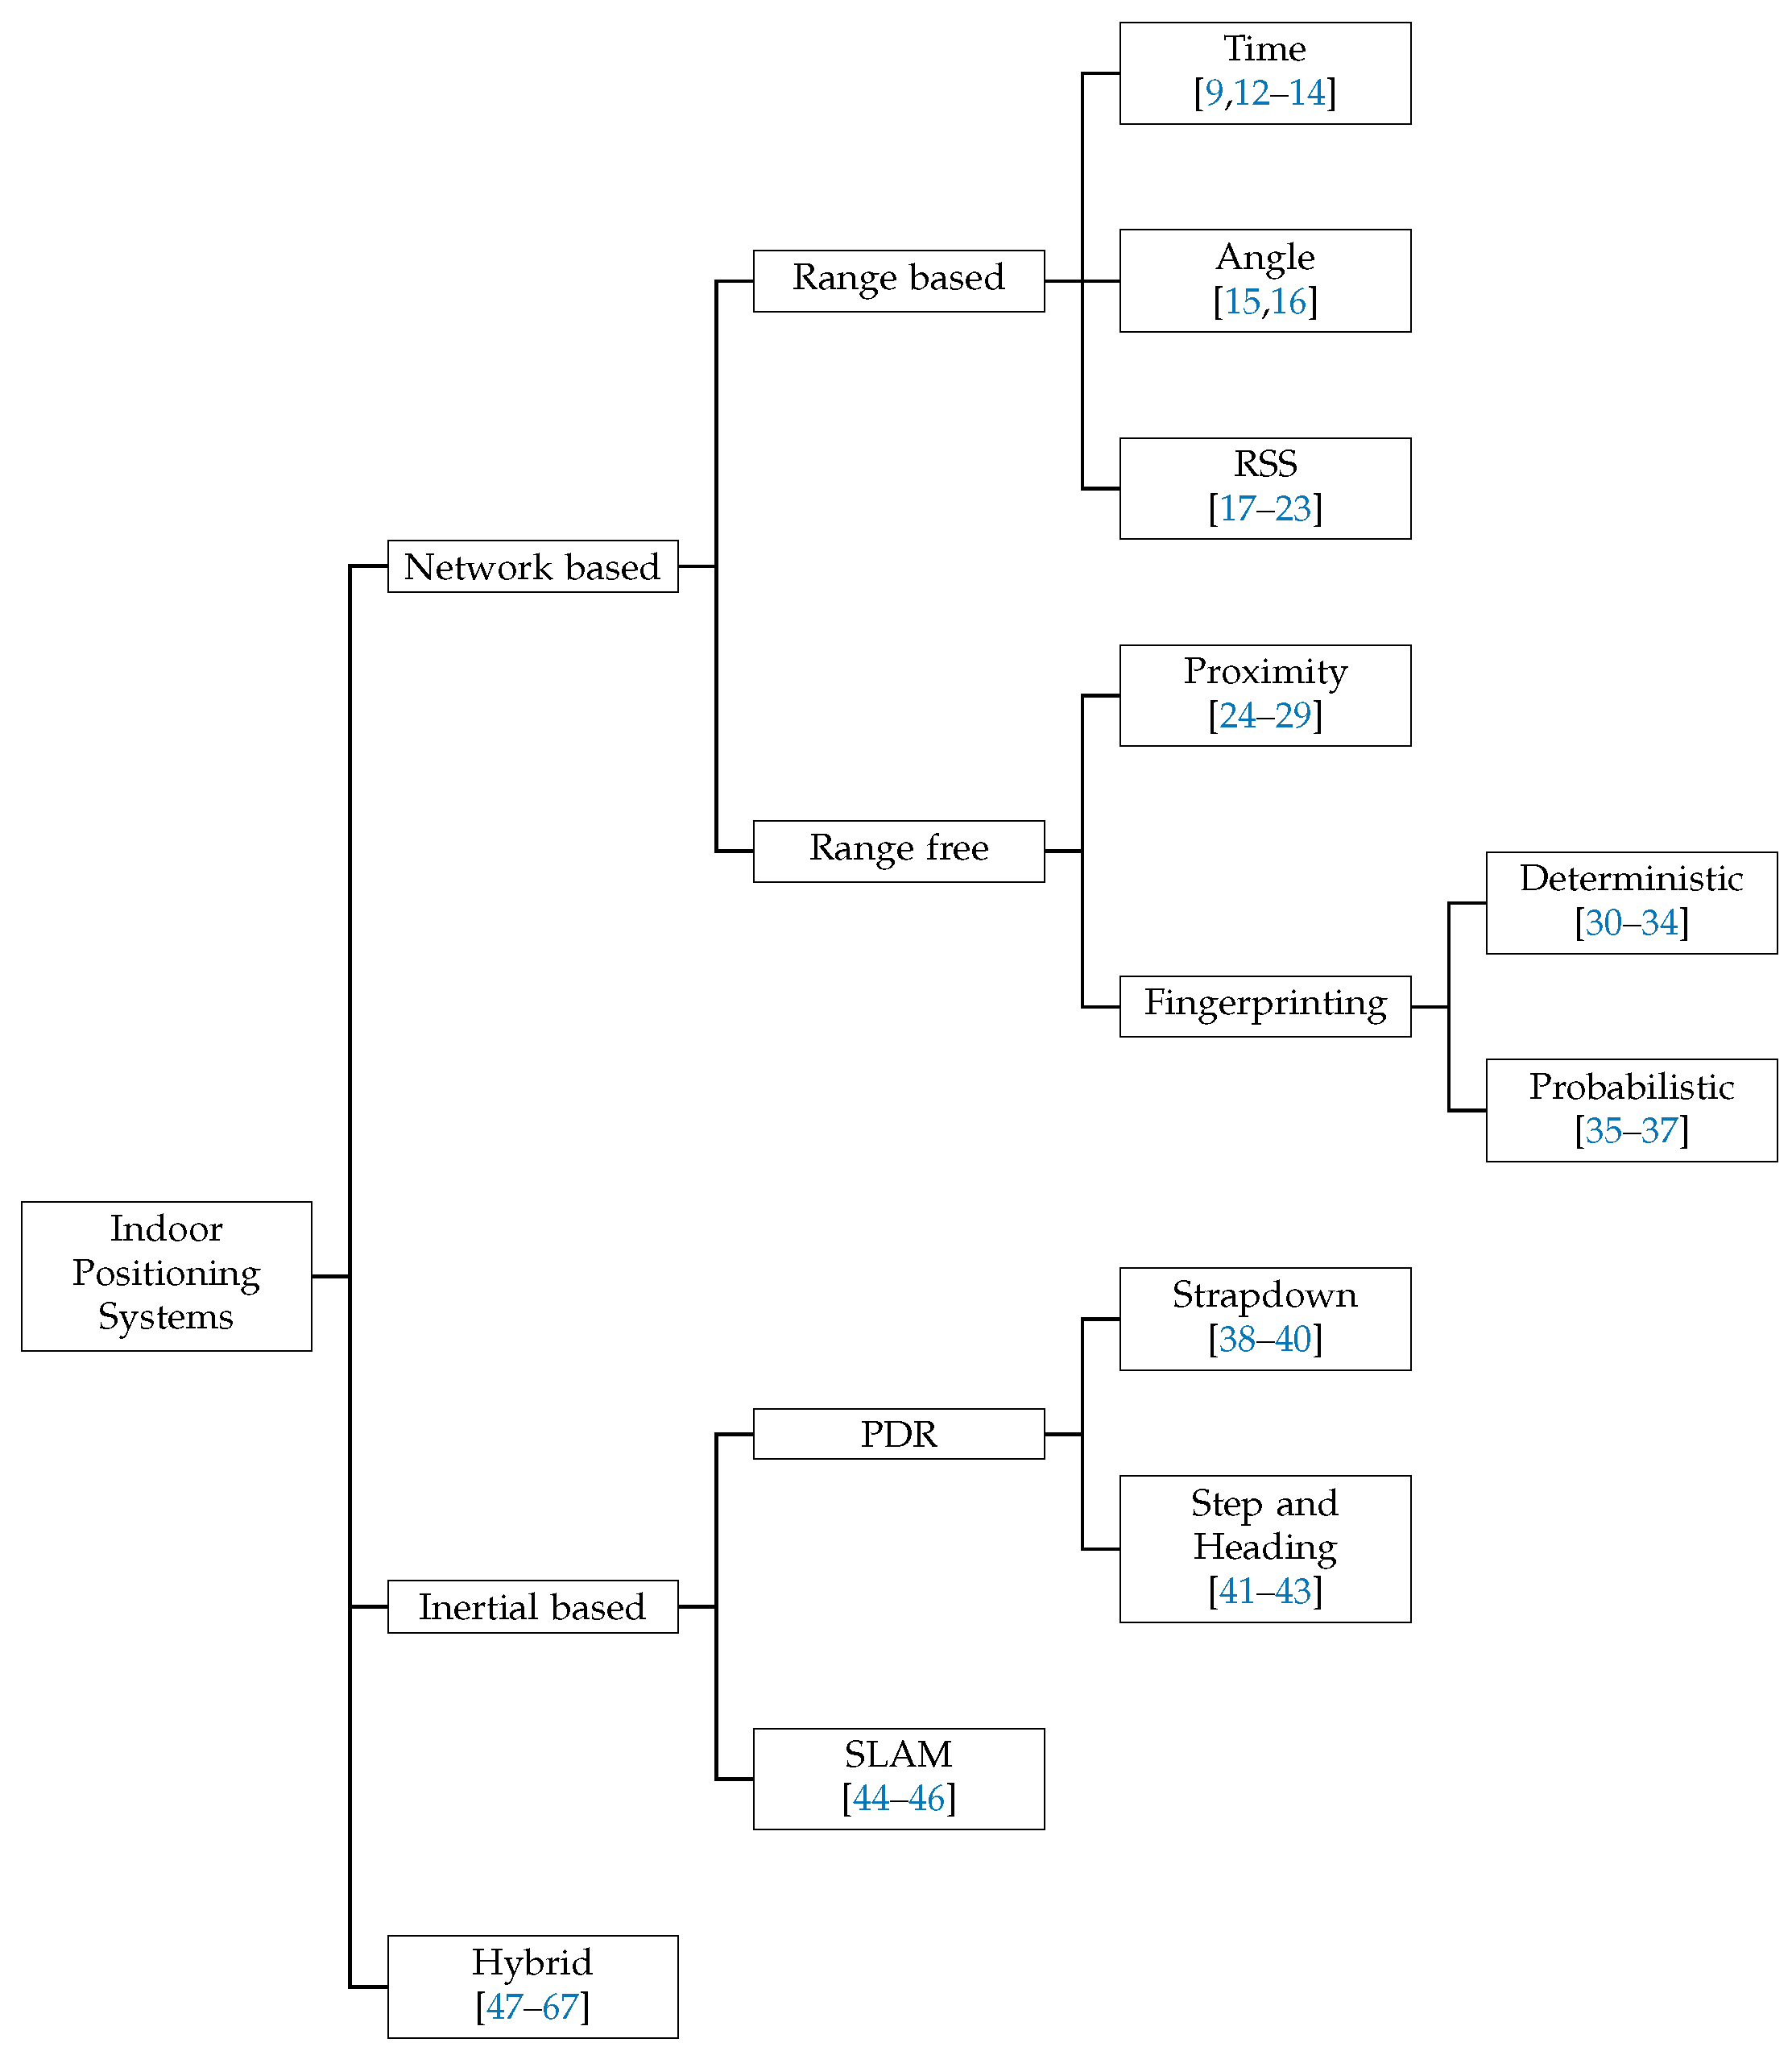
\includegraphics[width=0.7\textwidth]{../fig/ips}
	\caption[Classification of Indoor Positioning Systems]{Classification of Indoor Positioning Systems \citep[p. 2]{Correa2017}}
	\label{fig:ips}
\end{figure}

\citet{Correa2017} has classified indoor positioning systems into three groups: network based systems, inertial based systems, and hybrid systems.
Network based systems are built on wireless networks placed in the building and uses information from the wireless signals to estimate the position of the user who carries a wireless device.
Inertial based systems estimates the position of the user using self-contained sensors that measures the motions of the user relative to a starting point. 
Hybrid systems combine techniques from the other categories to estimate the position of the user.
Figure~\ref{fig:ips} is an overview of the classification taxonomy created by \citet{Correa2017}.
This research uses a network based IPS.

There are several ways of using Bluetooth Low Energy (BLE) beacons for positioning.
Normally the beacons are placed as anchors in the area the IPS is supposed to cover, and a device with a Bluetooth receiver is used to collect the signals transmitted from the beacons.
The collected signals are then used to calculate the position.
Depending on the availability of beacons and accuracy needed from the IPS the setup could use one beacon in each room, or multiple beacons in each room.

If one beacon in each room is used, the tracking device can read the received signal strength from all beacons in it's vicinity, and assume that the strongest signal strength must be from the closest beacon.
Therefore the tracking device can assume that it is located in the same room as the beacon which sent the strongest signal.
This could then be used to visualize and present the device's location, for the user, on a map.

If several beacons are placed in each room, one approach would be to use trilateration to determine the position.
Trilateration is a trigonometric method of positioning an object.
It requires the tracked object to have a line of sight to at least three beacons simultaneously.
The distance from each of the three beacons to the object must be calculated.
The position of the object is then the intersection of three circles, each centered at one of the three beacons \citep{Chawathe}.

\begin{figure}[h]
	\centering
	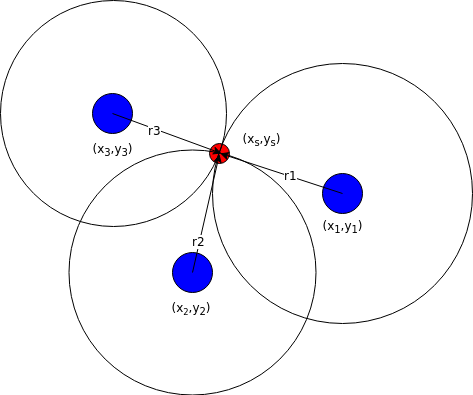
\includegraphics[width=0.8\textwidth]{../fig/Trilaterering}
	\caption{Trilateration: Three blue beacons with the distances $r1$, $r2$, and $r3$ to a red point}
	\label{fig:trilateration}
\end{figure}

Figure~\ref{fig:trilateration} illustrates an example of trilateration.
The blue dots are BLE beacons with a known position, and the red dot is the object with an unknown position.
The calculated distances from each beacon to the object are used as the radius of the circles around each beacon.
The position of the object can then be determined using trigonometric methods.

The problem with using trilateration for positioning is that it requires the computation of the distance between the beacon and the receiver using the signal strength.
According to \citet{Chawathe} the correlation between the received signal strength index and the distance between the objects is not sufficiently high enough to be used to determine an exact position.

Another approach to positioning with multiple beacons in the same room is using the nearest-neighbor algorithm \citep{Takahashi2016}.
Using this algorithm \citet{Takahashi2016} present a maximum error distance of 2.0m.
This algorithm requires the average RSSI, of 50 samples, from each beacon to be measured at predefined positions to be measured before the tracking starts.
It also requires the average RSSI, of 50 samples, to determine a position during the tracking \citep{Takahashi2016}.
These requirements makes this approach unsuitable for temporary setups, and for tracking moving objects.


\section{Related studies} 
This section presents a review of previous research that has relevance to the study presented in this thesis.
The selection criteria are that they:
\begin{itemize}
	\item Use Bluetooth for indoor positioning
	\item Enable firefighters to use data to improve efficiency
	\item Enable firefighter supervisors to plan work
\end{itemize}

\subsection{Bluetooth tracking of humans in an indoor environment: An application to shopping mall visits}
\label{sec:ble-tracking-mall}
\citet{Oosterlinck2017} investigated the applicability of indoor Bluetooth tracking in a shopping mall, and how it could be used for marketing purposes.
In their study \citep{Oosterlinck2017} found that Bluetooth tracking is usable to analyze the spatio-temporal behavior of the customers in the shopping mall.
They also found that the collected data is richer and of higher quality than traditional surveys used to collect information about customers movements, and therefore it could be useful for marketing purposes.
Their study relates to this thesis by using Bluetooth Low Energy technology for tracking humans, but in another situation and by using a slightly different approach.

\subsection{CoenoFire: Monitoring Performance Indicators of Firefighters in Real-world Missions using Smartphones}
In this research \citet{Feese2013} developed a smartphone based sensing system for monitoring temporal and behavioral performance in firefighting missions.
Their goal was to use the collected data to compare the performance metrics of one firefighter team with other firefighter teams participating in the same mission.
They used sensors on smartphones to sample data which was stored on the smartphone and transmitted the data so it could be used for real-time monitoring.
CoenoFire utilizes smartphones to monitor and firefighters, which is also what the research reported in this thesis does.

\subsection{Designing a Tangible Interface for Manager Awareness in Wilderness Search and Rescue}
In their research \citet{Jones2018} presents a tangible interface for supporting wilderness search-and-rescue managers.
The use case for this interface is a search-and-rescue operation involving multiple rescue teams. 
During the operation the interface will represent information about the makeup of the search area, the positions of the search teams, and the weather in the search area.
The intention is to present this information to the search-and-rescue managers, so they can use it in the planning of the operation.
Their study aims to track and monitor the movements of firefighters, but in another context, and using different technologies, than this thesis.

\subsection{Accurate indoor positioning of firefighters using dual foot-mounted inertial sensors and inter-agent ranging}
\citet{Nilsson2014} have developed a real-time localization systems which utilizes foot-mounted inertial sensors and RF-based communication to position firefighters.
Their results indicate that the system could provide a position accuracy of two to three meters in a realistic firefighter operation.
Their system also aims to track the positions of firefighters, but unlike the research presented in this thesis their goal is to use it in real missions, and the chosen technology is different.

\section{Summary}
In this chapter learning analytics was introduced, an overview of existing positioning systems was given, and four similar research projects were described.

\blankpage
\end{document}
